\chapter{MARCO TEÓRICO}
\label{ch:marco-teorico}
\thispagestyle{empty}

Este capítulo reúne las bases teóricas que sostienen el problema, el artefacto y su evaluación, y precisa los términos que se usarán. Integra los métodos de ampacidad, la heterogeneidad térmica, las PINN y la ciencia del diseño para conectar el problema formulado en la sección~\ref{sec:planteamiento-problema} con el modelo físico y la metodología. Los antecedentes bibliográficos se presentan en la Sección~\ref{sec:antecedentes}.

\section{BASES TEÓRICAS}
\label{sec:bases-teoricas}

Las bases teóricas comprenden las bases conceptuales del problema (Sección~\ref{sec:bases-conceptuales}) y las técnicas aplicadas (Sección~\ref{sec:tecnicas-aplicadas}).

\subsection{BASES CONCEPTUALES DEL PROBLEMA}
\label{sec:bases-conceptuales}

Las bases conceptuales explican el problema abstracto que sostiene el estudio: estimar un campo térmico en un dominio multimaterial, con fuentes, contornos e interfaces, para derivar una restricción operativa de corriente. Por tanto, esta sección no describe solo el cable, sino la relación física que convierte la heterogeneidad del entorno en cambios de $\Tmax$ e $\Imax$.

\subsubsection{GENERACIÓN Y EVACUACIÓN DE CALOR EN CABLES}
\label{subsec:generacion-evacuacion-calor}

La teoría de conducción parte de una relación simple: el calor fluye desde zonas de mayor temperatura hacia zonas de menor temperatura. En un medio heterogéneo, esa relación depende de la conductividad local, por lo que el flujo no puede explicarse solo con un promedio global de material \parencites{carslaw1959conduction,kakac2018heatConduction,hahn2012heatConduction}.

\begin{formula}[htbp]
\centering
\begin{equation}
\label{for:fourier-heterogeneo}
\mathbf{q}_{\mathrm{cond}}(x,y)=-k(x,y)\nabla T(x,y).
\end{equation}
\caption{Ley de Fourier para conducción en un medio heterogéneo. Fuente: Elaboración propia.}
\end{formula}

La Fórmula~\ref{for:fourier-heterogeneo} muestra por qué $\kx$ es un campo físico central del modelo. Si una región cercana al cable tiene baja conductividad, el flujo térmico encuentra mayor resistencia local; en cambio, si el suelo de relleno tiene alta conductividad, la disipación puede mejorar. Esta lógica fundamenta los parámetros de contraste, extensión y proximidad documentados en el \ref{anx:diseno-casos}; ninguno de ellos se clasifica como variable independiente de construcción del artefacto.

La Figura~\ref{fig:cadena-termica-metodologica} sintetiza esa relación para facilitar la lectura del marco teórico. La cadena inicia con la distribución espacial de conductividad, pasa por el flujo de calor y termina en la ampacidad, pero solo produce evidencia útil si el artefacto se verifica con métricas trazables.

\begin{figure}[htbp]
\centering
\resizebox{0.96\textwidth}{!}{%
\begin{tikzpicture}[
  node distance=0.72cm,
  bloque/.style={draw, rounded corners=3pt, align=center, text width=2.75cm,
                 minimum height=1.18cm, font=\small, line width=0.45pt},
  control/.style={bloque, text width=4.30cm, minimum height=1.05cm},
  arr/.style={-{Stealth[length=2.5mm]}, thick},
  feed/.style={-{Stealth[length=2.5mm]}, thick, dashed}
]
\node[bloque, fill=lightblue] (k) {Conductividad espacial\\$\kx$\\$C_k$, $f_h$, $d_h$};
\node[bloque, fill=green!12, right=of k] (q) {Flujo de calor\\$\mathbf{q}_{\mathrm{cond}}=-k\nabla T$};
\node[bloque, fill=green!12, right=of q] (t) {Campo térmico\\$T(x,y)$};
\node[bloque, fill=orange!15, right=of t] (tm) {Condición crítica\\$\Tmax$\\punto caliente};
\node[bloque, fill=orange!20, right=of tm] (i) {Resultado operativo\\$\Imax$\\margen térmico};
\node[control, fill=lightgray, below=0.82cm of t] (v) {Verificación DSR\\error, residuo, balance de energía, robustez y trazabilidad};
\draw[arr] (k) -- (q);
\draw[arr] (q) -- (t);
\draw[arr] (t) -- (tm);
\draw[arr] (tm) -- (i);
\draw[feed] (v.west) -| (q.south);
\draw[feed] (v.north) -- (t.south);
\draw[feed] (v.east) -| (tm.south);
\end{tikzpicture}
}
\caption{Cadena física y metodológica entre heterogeneidad térmica, campo de temperatura y ampacidad. Fuente: Elaboración propia.}
\label{fig:cadena-termica-metodologica}
\end{figure}

Las pérdidas eléctricas se transforman en calor y elevan la temperatura hasta que el calor generado por las pérdidas se equilibra con la disipación térmica hacia el entorno. En una sección 2D estacionaria, \textcite[752--760]{neher1957} relacionan esas pérdidas con resistencias térmicas y elevación de temperatura; a su vez, IEC 60287 formaliza el cálculo de corriente admisible para condiciones de régimen \parencite[cláusulas 4--5]{iec60287}. La temperatura límite del aislamiento convierte este problema de campo en una restricción de operación.

Una PDE describe una función desconocida mediante sus derivadas respecto de más de una coordenada matemática independiente. En este problema, la función desconocida es la temperatura y las coordenadas son las posiciones espaciales y, si el proceso es transitorio, el tiempo. Esta terminología matemática no corresponde a VI1--VI4 de la operacionalización metodológica. Por tanto, el modelo debe distinguir acumulación térmica, flujo por conducción y fuentes internas \parencites{carslaw1959conduction,kakac2018heatConduction,hahn2012heatConduction}.

En su forma dependiente del tiempo, la conducción de calor incorpora la inercia térmica del cable y del suelo. Para una sección 2D con propiedades espaciales, la ecuación puede escribirse como una adaptación directa de la ecuación clásica de calor en medios heterogéneos \parencites{carslaw1959conduction,kakac2018heatConduction,hahn2012heatConduction}:

\begin{formula}[htbp]
\centering
\begin{equation}
\label{for:calor-transitorio}
\rho(x,y)c_p(x,y)\,\frac{\partial T(x,y,t)}{\partial t}
=
\frac{\partial}{\partial x}\!\left(k(x,y)\frac{\partial T}{\partial x}\right)
+\frac{\partial}{\partial y}\!\left(k(x,y)\frac{\partial T}{\partial y}\right)
+Q(x,y,t),
\end{equation}
\caption{Ecuación de conducción de calor 2D transitoria. Fuente: Elaboración propia.}
\end{formula}

En la Fórmula~\ref{for:calor-transitorio}, $\rho$ representa la densidad de masa y $\rho c_p$ la capacidad térmica volumétrica. Este símbolo no debe confundirse con la resistividad térmica, que en el documento se denota $\rhoth$. Además, $k(x,y)$ controla la disipación local y $Q(x,y,t)$ agrupa las fuentes internas. En cambio, IEC 60853 conserva el término transitorio para tratar ciclos de carga y secado parcial \parencite[cláusulas 2--4]{iec60853}.

La forma estacionaria se obtiene cuando la acumulación térmica se anula, es decir, cuando $\partial T/\partial t=0$. En notación vectorial, el balance queda:

\begin{formula}[htbp]
\centering
\begin{equation}
\label{for:calor-estacionario-marco}
\nabla\!\cdot\!\left(k(x,y)\nabla T(x,y)\right)+Q(x,y)=0,
\qquad (x,y)\in\Omega .
\end{equation}
\caption{Ecuación de conducción de calor 2D estacionaria en notación vectorial. Fuente: Elaboración propia.}
\end{formula}

La Fórmula~\ref{for:calor-estacionario-marco} usa la misma notación que la formulación metodológica de la Fórmula~\ref{for:calor}: $\kx$ representa la conductividad espacial y $Q(x,y)$ representa las pérdidas térmicas. Así, el marco teórico y la metodología comparten una única base física y simbólica.

Si corriente, temperatura ambiente o humedad cambian con el tiempo, el almacenamiento de calor afecta la respuesta térmica. Por ello, este efecto también aparece en revisiones de DTR para cables enterrados \parencites[3--6]{enescu2021}[14843--14845]{fariz2026}.

La ampacidad no es una propiedad fija del cable aislado. Cambia con temperatura ambiente, profundidad, separación, configuración, pérdidas, conductividad y humedad, variables destacadas en revisiones técnicas y estudios de suelo \parencites[3--6]{enescu2021}[1,6--9]{khumalo2025}. Por ello, dos cables iguales pueden tener capacidades diferentes si el camino térmico de sus instalaciones difiere. En la metodología, esta idea se convierte en la condición de búsqueda de $\Imax$ de la Fórmula~\ref{for:ampacidad}.

La Figura~\ref{fig:cable-multicapa}, tomada de \textcite[fig.~2]{kim2025}, concreta la primera escala del objeto de estudio. En el cable, el conductor, las pantallas, el aislamiento XLPE, la cubierta y las capas metálicas no solo cumplen funciones eléctricas, sino que también aportan fuentes y resistencias térmicas. Esta estructura interna explica por qué el campo de temperatura debe leerse como una respuesta multicapa y no como la temperatura de un sólido homogéneo.

\begin{figure}[htbp]
\centering
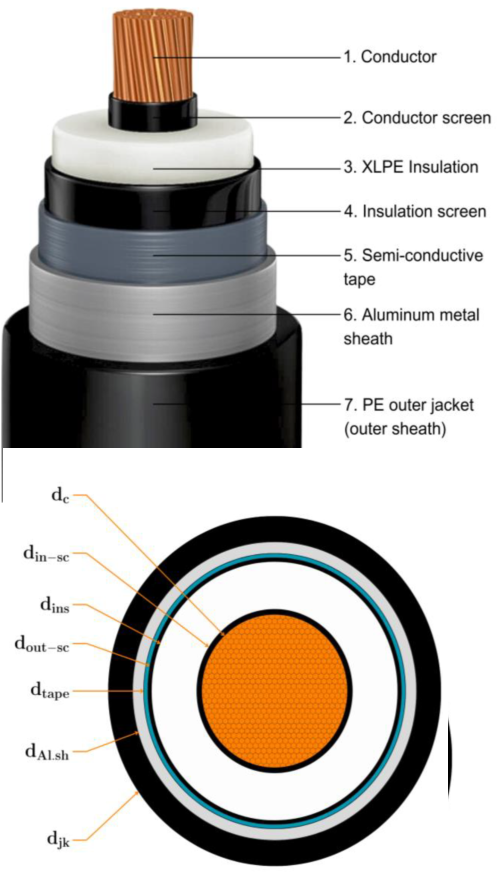
\includegraphics[height=0.27\textheight,keepaspectratio]{kim2025_cable_xsection}
\caption[Estructura multicapa de un cable XLPE]{Estructura multicapa de un cable XLPE usado como referencia del objeto de estudio. Fuente: \textcite[fig.~2]{kim2025}.}
\label{fig:cable-multicapa}
\end{figure}

La Figura~\ref{fig:zanja-cable}, basada en \textcite[fig.~1]{enescu2021}, muestra la segunda escala del objeto de estudio: la instalación enterrada. Allí el cable queda acoplado al suelo de relleno, al lecho de asiento cuando existe y al suelo nativo. Por ello, la conductividad térmica espacialmente variable $\kx$ no pertenece únicamente al cable, sino al arreglo de cables--entorno térmico, y debe representar la posición relativa de materiales con conductividades distintas.

\begin{figure}[htbp]
\centering
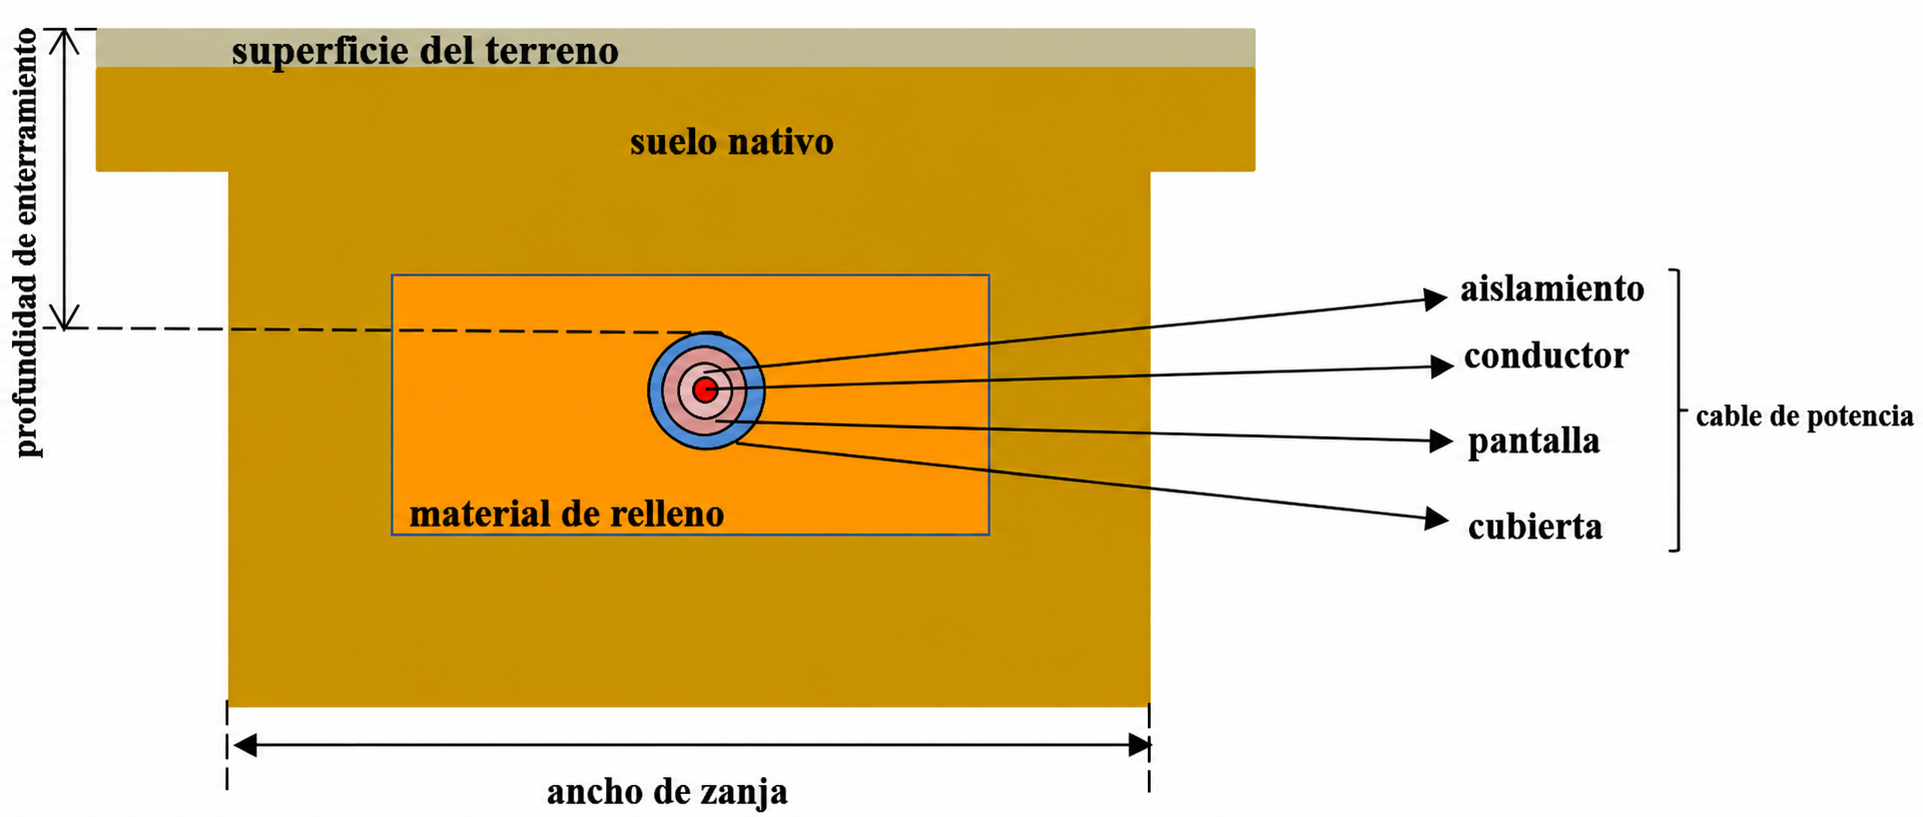
\includegraphics[width=0.97\textwidth,height=6.8cm,keepaspectratio]{enescu_trench_xsection_es}
\caption[Zanja y entorno térmico del cable enterrado]{Zanja y entorno térmico del cable enterrado: suelo de relleno, suelo nativo, profundidad de instalación y capas principales del cable. Fuente: \textcite[fig.~1]{enescu2021}.}
\label{fig:zanja-cable}
\end{figure}

\subsubsection{CONDUCTIVIDAD, RESISTIVIDAD Y HETEROGENEIDAD}
\label{subsec:conductividad-heterogeneidad}

La conductividad térmica $k$ expresa la facilidad para transferir calor, mientras que la resistividad térmica $\rhoth$ expresa la oposición del material a esa transferencia. Para un material homogéneo e isotrópico son magnitudes inversas:

\begin{equation}
\label{for:conductividad-resistividad}
\rhoth=\frac{1}{k},
\qquad
k=\frac{1}{\rhoth}.
\end{equation}

Por ello, una mayor resistividad térmica equivale a una menor conductividad y a una mayor dificultad para evacuar calor. En suelos, ambas propiedades dependen de la composición, la densidad y el contenido de agua; el aumento de resistividad por secado observado por \textcite[1,7]{khumalo2025} muestra que puede formarse una zona local que actúa como barrera. La literatura de cables suele reportar $\rhoth$ en \si{\kelvin\metre\per\watt}, mientras que la PDE de esta investigación usa su inversa $k$ en \si{\watt\per\metre\per\kelvin}. Toda conversión entre valores publicados y entradas del modelo aplicará la Fórmula~\ref{for:conductividad-resistividad}. El valor usado para diseño debe representar el estado de instalación y seguir procedimientos normalizados cuando proviene de ensayos o fuentes técnicas \parencite[secciones 4--6]{ieee442}.

Una propiedad promedio conserva cierta cantidad global, pero no necesariamente conserva la temperatura máxima ni la ubicación del punto caliente. Dos mapas con el mismo promedio pueden producir rutas de flujo distintas si una región aislante se ubica junto al cable o lejos de él. Esta es la razón física para estudiar $C_k$, $f_h$ y $d_h$ como dimensiones separadas.

Las interfaces también son parte del problema teórico. Cuando dos materiales están en contacto, el modelo debe conservar temperatura y flujo normal, salvo que se declare una resistencia de contacto. Esta condición, formulada en la Fórmula~\ref{for:interfaz}, evita que el cambio de material produzca saltos no físicos en el campo térmico \parencites{carslaw1959conduction,kakac2018heatConduction}{patankar1980numerical}[3]{xing2023}.

La Tabla~\ref{tab:base-teorica-uso} resume cómo estas bases se usan en otras partes del documento. Por tanto, el marco teórico cumple una función de enlace: explica la teoría y muestra cómo esa teoría se convierte en variables, fórmulas, métricas y anexos.

\begin{table}[htbp]
\centering
\caption{Relación entre base teórica y uso metodológico. Fuente: Elaboración propia.}
\label{tab:base-teorica-uso}
\begingroup
\footnotesize
\setlength{\tabcolsep}{3pt}
\renewcommand{\arraystretch}{1.25}
\begin{tabularx}{\textwidth}{L{3.2cm}Y Y}
\toprule
\textbf{Base teórica} & \textbf{Relación física} & \textbf{Uso en el estudio} \\
\midrule
Conductividad $\kx$ y resistividad $\rhoth$ & Son magnitudes inversas; $k$ controla el flujo de calor local según la ley de Fourier. & Los datos en $\rhoth$ se convierten a $k$ antes de parametrizar el paquete inicial $P_1$, los escenarios $E_3$ y las comparaciones $C_4$ descritos en la sección~\ref{sec:dimensiones-operativas} y el \ref{anx:diseno-casos}. \\
Campo $T(x,y)$ & Solución de la ecuación de conducción para una geometría, fuentes y contornos dados. & Salida numérica del artefacto e indicador contenido en VD3 y VD4; no constituye por sí solo una variable metodológica. \\
Temperatura máxima $\Tmax$ & Restricción térmica que resume la condición crítica del conductor. & Indicador de VD2--VD4 y criterio de error en la Fórmula~\ref{for:metricas-evaluacion}. \\
Ampacidad $\Imax$ & Corriente máxima compatible con el límite térmico adoptado. & Resultado operativo calculado con la condición de la Fórmula~\ref{for:ampacidad}. \\
Interfaces térmicas & Conservan temperatura y flujo entre materiales. & Requisito físico del artefacto y parte de la verificación de la sección~\ref{subsec:verificacion-dsr}. \\
\bottomrule
\end{tabularx}
\endgroup
\end{table}

\subsubsection{MÉTODOS DE CÁLCULO TÉRMICO}
\label{subsec:metodos-calculo-termico}

Los circuitos térmicos son rápidos e interpretables, pero requieren equivalencias geométricas, por lo que las revisiones de cables los distinguen de los métodos de solución de campo térmico \parencite[4--6]{enescu2021}. Los métodos numéricos de campo resuelven la PDE sobre una malla, una grilla o una partición del dominio. FEM aproxima la solución por elementos; FDM reemplaza derivadas por diferencias en una grilla; FVM integra balances sobre volúmenes de control y conserva flujos locales \parencites{patankar1980numerical}[3--4,93--99]{cigre2025}.

Estos métodos son útiles porque representan geometría, materiales, fuentes y contornos con mayor detalle que una equivalencia térmica global. Sin embargo, su credibilidad depende de propiedades, condiciones de borde, discretización, convergencia y verificación. Las PINN aproximan la solución con una red y diferenciación automática, pero trasladan parte de la dificultad a muestreo, ponderación de pérdidas y optimización \parencites[3--4,93--99]{cigre2025}[1--2,14--17]{lawal2022}.

Los métodos se tratarán como complementarios. Las normas IEC aportarán la referencia normativa, los casos FEM aportarán la referencia numérica del campo térmico y la PINN será el artefacto investigado. Por tanto, una discrepancia no se interpretará automáticamente como error de IEC o superioridad de PINN. Primero se revisarán supuestos, dominio y evidencia.

La Tabla~\ref{tab:metodos-calculo-termico} organiza esa complementariedad. Esta síntesis es importante porque la metodología no elige un método por preferencia, sino por función: norma para línea base, métodos de campo para referencia, casos analíticos para verificación y PINN como artefacto evaluado.

\begin{table}[htbp]
\centering
\caption{Función de los métodos térmicos dentro del estudio. Fuente: Elaboración propia a partir de \textcite{iec60287}, \textcite{iec60853}, \textcite[4--6]{enescu2021}, \textcite[3--4,93--99]{cigre2025}, \textcite{patankar1980numerical} y \textcite{raissi2019}.}
\label{tab:metodos-calculo-termico}
\begingroup
\footnotesize
\setlength{\tabcolsep}{3pt}
\renewcommand{\arraystretch}{1.25}
\begin{tabularx}{\textwidth}{L{3.1cm}Y Y}
\toprule
\textbf{Método o referencia} & \textbf{Aporte principal} & \textbf{Límite que justifica la evaluación} \\
\midrule
IEC y circuitos térmicos & Dan una base normativa e interpretable para corriente admisible. & Requieren equivalencias térmicas y pueden ocultar heterogeneidades locales. \\
Soluciones analíticas o manufacturadas & Permiten verificar el código frente a respuestas conocidas. & Cubren geometrías y condiciones idealizadas. \\
FEM & Representa geometría, materiales y contornos con detalle espacial. & Exige malla, convergencia y repetición del modelo para cada escenario. \\
FDM & Aproxima las derivadas de la PDE mediante diferencias en una grilla. & Es directo en dominios regulares, pero pierde flexibilidad ante geometrías e interfaces complejas. \\
FVM & Integra balances de energía sobre volúmenes de control. & Conserva flujos locales, pero requiere tratamiento cuidadoso de interfaces y contornos. \\
PINN & Integra PDE, contornos, interfaces y datos de referencia en una pérdida común. & Requiere controlar entrenamiento, pesos de pérdida, puntos de colocación y robustez. \\
\bottomrule
\end{tabularx}
\endgroup
\end{table}

\subsection{TÉCNICAS APLICADAS}
\label{sec:tecnicas-aplicadas}

\subsubsection{REDES NEURONALES INFORMADAS POR LA FÍSICA}
\label{subsec:pinn}

Una PINN, según la formulación de \textcite[686--690]{raissi2019}, representa una variable física mediante una red neuronal y usa diferenciación automática para calcular las derivadas que aparecen en la PDE. Los puntos de colocación permiten evaluar el residuo sin requerir una etiqueta de temperatura en cada punto. Si existen observaciones, pueden añadirse como otro término y convertir el problema en una combinación física--datos.

La Figura~\ref{fig:arquitectura-pinn-lawal} muestra esta organización en una arquitectura PINN convencional. A la izquierda se encuentra una red neuronal directa que recibe las coordenadas independientes y aproxima las variables físicas. A la derecha, las salidas de la red pasan por operadores de diferenciación automática para construir el residuo $f$ de la ecuación gobernante. El entrenamiento reúne entonces una pérdida asociada con los datos y otra asociada con la física. Así, la información física no constituye una capa adicional de neuronas: actúa como una restricción sobre las funciones que la red puede aprender.

\begin{figure}[H]
\centering
\resizebox{0.94\textwidth}{!}{%
\begin{tikzpicture}[
  font=\small,
  neurona/.style={circle, draw, minimum size=9mm, inner sep=1pt, line width=0.45pt},
  entrada/.style={neurona, fill=lightblue},
  oculta/.style={neurona, fill=lightgray},
  salida/.style={neurona, fill=yellow!55},
  operador/.style={neurona, fill=red!15, minimum size=10.5mm, inner sep=0.5pt,
                   font=\footnotesize, align=center},
  bloque/.style={draw, rounded corners=3pt, align=center, minimum height=10mm,
                 text width=2.35cm, line width=0.45pt},
  grupo/.style={draw=gray!75, fill=lightgray!55, dashed, rounded corners=7pt,
                inner sep=7pt, line width=0.55pt},
  enlace/.style={-{Stealth[length=1.8mm]}, draw=gray!60, line width=0.32pt},
  fisica/.style={-{Stealth[length=2mm]}, draw=gray!75, line width=0.48pt},
  perdida/.style={-{Stealth[length=2.4mm]}, draw=gray!80, dashed, line width=0.9pt}
]
  % Entradas
  \node[entrada] (x) at (0,2.1) {$x$};
  \node[entrada] (y) at (0,0.7) {$y$};
  \node[entrada] (t) at (0,-0.7) {$t$};

  % Capas ocultas
  \node[oculta] (h11) at (2.25,2.55) {$\sigma$};
  \node[oculta] (h12) at (2.25,1.25) {$\sigma$};
  \node[oculta] (h13) at (2.25,-0.05) {$\sigma$};
  \node[oculta] (h14) at (2.25,-1.35) {$\sigma$};
  \node[oculta] (h21) at (3.75,2.55) {$\sigma$};
  \node[oculta] (h22) at (3.75,1.25) {$\sigma$};
  \node[oculta] (h23) at (3.75,-0.05) {$\sigma$};
  \node[oculta] (h24) at (3.75,-1.35) {$\sigma$};

  % Salidas de la red
  \node[salida] (u) at (5.55,1.45) {$u$};
  \node[salida] (v) at (5.55,-0.25) {$v$};

  % Operadores físicos y residuo
  \node[operador] (id)  at (7.55,2.75) {$I$};
  \node[operador] (dx)  at (7.55,1.40) {$\partial/\partial x$};
  \node[operador] (dy)  at (7.55,0.05) {$\partial/\partial y$};
  \node[operador] (dxx) at (7.55,-1.30) {$\partial^2/\partial x^2$};
  \node[operador] (dyy) at (7.55,-2.65) {$\partial^2/\partial y^2$};
  \node[bloque, fill=yellow!20, text width=1.45cm] (f) at (9.85,0.25) {Residuo\\$f$};

  % Pérdidas
  \node[bloque, fill=yellow!45, text width=3.15cm] (ldata) at (5.30,-3.85)
    {Pérdida de datos\\[0.15em]$\mathcal{L}_{\mathrm{datos}}$};
  \node[bloque, fill=yellow!20, text width=3.15cm] (lphysics) at (10.00,-3.85)
    {Pérdida física\\$\mathcal{L}_{\mathrm{física}}$};
  \node[bloque, fill=lightblue, text width=3.15cm] (ltotal) at (7.65,-5.15)
    {Pérdida total\\$\mathcal{L}_{\mathrm{total}}$};

  % Conexiones densas de la red neuronal
  \foreach \a in {x,y,t}
    \foreach \b in {h11,h12,h13,h14}
      \draw[enlace] (\a) -- (\b);
  \foreach \a in {h11,h12,h13,h14}
    \foreach \b in {h21,h22,h23,h24}
      \draw[enlace] (\a) -- (\b);
  \foreach \a in {h21,h22,h23,h24}
    \foreach \b in {u,v}
      \draw[enlace] (\a) -- (\b);

  \foreach \a in {u,v}
    \foreach \b in {id,dx,dy,dxx,dyy}
      \draw[fisica] (\a) -- (\b);
  \foreach \a in {id,dx,dy,dxx,dyy}
    \draw[fisica] (\a) -- (f);

  \draw[perdida] (v.south) -- ++(0,-0.40cm) -| (ldata.north);
  \draw[perdida] (f.south) -- (lphysics.north);
  \draw[fisica, line width=0.8pt] (ldata.south) -- (ltotal.west);
  \draw[fisica, line width=0.8pt] (lphysics.south) -- (ltotal.east);

  % Agrupaciones conceptuales sobre una capa de fondo
  \begin{scope}[on background layer]
    \node[grupo, fit=(x)(y)(t)] (ginput) {};
    \node[grupo, fit=(h11)(h14)(h21)(h24)] (gred) {};
    \node[grupo, fit=(u)(v)] (gout) {};
    \node[grupo, fit=(id)(dyy)(f)] (gphysics) {};
  \end{scope}
  \node[font=\bfseries\small, above=1mm of gred.north] {Red neuronal};
  \node[font=\bfseries\small, above=1mm of gphysics.north] {Informada por física};
\end{tikzpicture}%
}
\caption[Arquitectura general de una red neuronal informada por física]{Arquitectura general de una red neuronal informada por física: la red aproxima las variables de salida y la diferenciación automática permite evaluar las derivadas y el residuo de la ecuación gobernante; las pérdidas de datos y física se combinan durante el entrenamiento. Fuente: \textcite[fig.~1]{lawal2022}.}
\label{fig:arquitectura-pinn-lawal}
\end{figure}

En términos de arquitectura, una PINN puede usar una red neuronal directa con entradas, capas ocultas, funciones de activación y una o varias salidas físicas, como $u$ y $v$ en la Figura~\ref{fig:arquitectura-pinn-lawal}. La propuesta fundacional de \textcite[686--690]{raissi2019} comparte los parámetros de la aproximación de la solución y del residuo físico: las derivadas no se estiman con una red separada, sino que se obtienen de la misma aproximación mediante diferenciación automática. Por ello, la diferencia central respecto de una red supervisada convencional no está solo en la arquitectura, sino en el entrenamiento, porque la pérdida incorpora la PDE, los contornos y, cuando existen, datos de referencia \parencites[686--690]{raissi2019}[1--2,14--17]{lawal2022}.

Para el problema térmico, la red no aprende solo una relación empírica entre entradas y salidas. Aprende una aproximación del campo $T(x,y)$ que debe reducir el incumplimiento local de la ecuación de conducción, de modo que el residuo físico se convierte en evidencia de consistencia del modelo \parencites[686--690]{raissi2019}[1--2,14--17]{lawal2022}. La Fórmula~\ref{for:residuo-pinn-calor} se obtiene al evaluar la ecuación de calor estacionaria con $T(x,y)$ y reordenar sus términos como residuo.

\begin{formula}[htbp]
\centering
\begin{equation}
\label{for:residuo-pinn-calor}
r_f(x,y)=
\nabla\!\cdot\!\left(k(x,y)\nabla T(x,y)\right)
+Q(x,y).
\end{equation}
\caption{Residuo físico de una PINN para conducción de calor 2D estacionaria. Fuente: Elaboración propia.}
\end{formula}

La Fórmula~\ref{for:residuo-pinn-calor} debe interpretarse junto con contornos, interfaces y datos de referencia, cuando existan. Por ello, la metodología usa una función de pérdida compuesta, presentada en la Fórmula~\ref{for:loss}, y no una única métrica de ajuste. En esa pérdida, $\mathcal{L}_{\mathrm{PDE}}$ se calcula con el residuo en puntos de colocación, mientras que los otros términos conectan la solución con contornos, interfaces, datos y conservación de energía. Esta distinción es importante porque el estudio evaluará dominios multimateriales, donde la representación de interfaces y el balance entre términos de pérdida pueden condicionar el entrenamiento \parencites[16]{pan2025}[2--6]{ren2025}.

La Figura~\ref{fig:esquema-pinn-calor} resume ese mecanismo para el problema térmico estacionario. Primero, la red recibe las coordenadas espaciales y los parámetros del caso; luego, produce una aproximación del campo $T(x,y)$. Después, la diferenciación automática calcula sus gradientes espaciales \parencite[686--690]{raissi2019}. Finalmente, la función de pérdida penaliza el incumplimiento de la ecuación de calor, los contornos, las interfaces y los datos disponibles, de modo que el esquema sintetiza \textcite[686--690]{raissi2019}, \textcite[1--2,14--17]{lawal2022} y \textcite[1,3,16]{pan2025}.

\begin{figure}[htbp]
\centering
\begin{tikzpicture}[
  font=\footnotesize,
  node distance=0.50cm and 0.36cm,
  stage/.style={draw, rounded corners=3pt, align=center, text width=2.30cm,
                minimum height=1.05cm, fill=white, line width=0.45pt},
  model/.style={stage, fill=lightgray},
  residual/.style={stage, fill=lightblue, text width=2.86cm,
                   minimum height=1.55cm},
  total/.style={stage, fill=lightgray, text width=2.62cm,
                minimum height=1.15cm},
  output/.style={stage, text width=2.62cm, minimum height=1.05cm},
  group/.style={draw, dashed, rounded corners=4pt, inner sep=4pt,
                line width=0.4pt},
  arr/.style={-{Stealth[length=2.4mm]}, line width=0.45pt},
  feed/.style={-{Stealth[length=2.4mm]}, line width=0.45pt, dashed,
               rounded corners=2pt}
]
\node[stage] (input) {Entradas\\$(x,y)$; $k,Q$\\contornos/datos};
\node[model, right=of input] (nn) {Red PINN\\capas ocultas\\activación\\$T(x,y)$};
\node[model, right=of nn] (auto) {Diferenciación\\automática\\$\nabla T,\nabla\!\cdot(k\nabla T)$};
\node[residual, right=of auto] (terms) {Pérdidas evaluadas\\[0.15em]
$r_f=\nabla\!\cdot(k\nabla T)+Q$\\
$r_b,r_i,r_d$};
\node[total, right=of terms] (loss) {Pérdida total\\$\mathcal{L}=\sum_j\lambda_j\mathcal{L}_j$};
\node[output, below=0.62cm of auto] (out) {Salida evaluada\\campo de temperatura\\$T(x,y)$\\$\Tmax$, punto caliente, $\Imax$};
\node[stage, below=0.62cm of loss] (opt) {Optimizador\\actualiza $\theta$};
\node[group, fit=(terms)(loss), label={[font=\scriptsize]above:Evaluación física y de datos}] (lossbox) {};
\coordinate (fbrail) at ($(out.south)+(0,-0.30cm)$);

\draw[arr] (input) -- (nn);
\draw[arr] (nn) -- (auto);
\draw[arr] (auto) -- (terms);
\draw[arr] (terms) -- (loss);
\draw[arr] (loss) -- (opt);
\draw[feed] (opt.south) |- (fbrail) -| (nn.south);
\draw[arr] (auto.south) -- (out.north);
\end{tikzpicture}
\caption[Esquema de funcionamiento de una PINN aplicada a conducción de calor]{Esquema de funcionamiento de una PINN aplicada a conducción de calor. Fuente: Elaboración propia a partir de \textcite{raissi2019}, \textcite{lawal2022} y \textcite{pan2025}.}
\label{fig:esquema-pinn-calor}
\end{figure}

Su utilidad para el estudio tiene tres razones: primero, ofrece una representación continua del campo; segundo, integra $\kx$; tercero, puede extenderse a identificación inversa. Sin embargo, sus riesgos también son claros, entre ellos el mal balance de pérdidas, las discontinuidades, los mínimos de optimización, la sensibilidad y la demanda computacional del entrenamiento \parencites[2--6]{ren2025}[16]{pan2025}.

Las técnicas de descomposición de dominio de \textcite[1--2]{shukla2021} aportan una ruta posible para tratar discontinuidades. Sin embargo, se incorporarán solo si el diseño básico demuestra que las necesita.

\subsubsection{CIENCIA DEL DISEÑO Y NATURALEZA DE LA CONTRIBUCIÓN}
\label{subsec:dsr-contribucion}

La metodología DSR busca conocimiento prescriptivo mediante artefactos útiles y evaluados. En este plan, el objeto físico es el arreglo de cables--entorno térmico bajo heterogeneidad.

El artefacto situado será el prototipo PINN usado para estudiar ese sistema. Además, la contribución abstracta incluirá requisitos, arquitectura, protocolo de evaluación y principios de diseño.

Estas categorías son coherentes con la tipología de \textcite[343--349]{gregor2013}. Por tanto, la investigación se posiciona como una mejora de métodos PINN aplicados a esta clase de problema.

Los principios iniciales son: conservar explícitamente la física; representar interfaces sin promediar de forma inadvertida; separar verificación de validación; mantener incertidumbre numérica por debajo del efecto analizado; y preservar trazabilidad de cada ejecución. Estos principios son proposiciones de diseño sujetas a evaluación y refinamiento, no conclusiones anticipadas.

En síntesis, el marco teórico reduce el problema a una cadena física: $\kx$ modifica el flujo térmico, el flujo determina $T(x,y)$ y $\Tmax$ limita la corriente admisible. Esta relación no define las variables metodológicas. La cadena metodológica está formada por objetos discretos y conserva cada producto: VI1--OE1--VD1, $\{\mathrm{VD1},R_2\}$--OE2--VD2, $\{\mathrm{VD2},E_3\}$--OE3--VD3 y $\{\mathrm{VD3},C_4\}$--OE4--VD4; después continúan la evaluación DSR y la síntesis de principios. Ambas cadenas sostienen la metodología del Capítulo~\ref{ch:metodologia} y la organización del \ref{anx:operacionalizacion-variables} y del \ref{anx:diseno-casos}.

\section{DEFINICIÓN DE TÉRMINOS}
\label{sec:definicion-terminos}

Esta sección precisa los términos que se usarán con sentido técnico u operacional en el estudio. Se incluyen aquellos que intervienen directamente en el problema, objetivos, hipótesis, dimensiones operativas, métricas o alcance del artefacto. Las definiciones tomadas de normas, literatura técnica o metodología DSR se citan; las definiciones operacionales se formulan para esta investigación y se apoyan en las fuentes que sustentan su uso.

\begingroup
\newcounter{terminodefinicion}
\renewcommand*\descriptionlabel[1]{\refstepcounter{terminodefinicion}\normalfont\bfseries\thesection.\theterminodefinicion. #1}
\begin{description}[style=nextline,itemsep=0.5\baselineskip,parsep=0pt,topsep=0.25\baselineskip]
  \item[Ampacidad.] Corriente máxima que puede transportar un cable sin superar el límite térmico adoptado para sus materiales y condiciones de instalación. Se denotará como $\Imax$ y se obtendrá al buscar la corriente que hace que $\Tmax$ alcance $T_{\mathrm{lim}}$ \parencites[752--760]{neher1957}{anders2005}[cláusulas 4--5]{iec60287}[3--6]{enescu2021}.

  \item[Ampacidad dinámica o DTR.] Estimación de la capacidad de corriente considerando la evolución temporal de carga, temperatura ambiente, suelo y estado térmico previo del cable. Se distingue de la ampacidad en régimen permanente porque aprovecha la inercia térmica del sistema y requiere supuestos transitorios explícitos \parencites[cláusulas 2--4]{iec60853}[3--6]{enescu2021}[14843--14845]{fariz2026}.

  \item[Artefacto.] Producto diseñado para resolver un problema relevante y generar conocimiento evaluable. Comprende la especificación, el prototipo PINN, los escenarios de prueba, las métricas y los principios de diseño derivados; se distingue del objeto de estudio físico, que es el arreglo de cables--entorno térmico \parencites[55--56]{peffers2007}[342--350]{gregor2013}.

  \item[Suelo de relleno.] Suelo colocado como relleno en la zanja alrededor del cable o sobre el lecho de asiento. Puede tener propiedades térmicas distintas a las del suelo nativo y modificar la evacuación de calor del arreglo de cables--entorno térmico \parencites{anders2005}[1--3]{atoccsa2024}[1,10,16]{kim2025}[secciones 4--6]{ieee442}.

  \item[Lecho de asiento.] Capa de material colocada inmediatamente debajo del cable dentro de la zanja. En el contexto del estudio se considera una región cercana al cable cuya conductividad, extensión y posición pueden afectar la temperatura máxima y el punto caliente \parencites[1--4]{oclon2015}[1,10,16]{kim2025}[secciones 4--6]{ieee442}.

  \item[Cable eléctrico enterrado.] Sistema multicapa instalado bajo tierra para transportar energía eléctrica. Su respuesta térmica depende de pérdidas internas, capas del cable, profundidad, configuración, suelo de relleno, suelo nativo y condiciones de frontera \parencites[752--760]{neher1957}{anders2005}[3--5]{enescu2020}[fig.~2]{kim2025}.

  \item[Caso de referencia o \textit{benchmark}.] Configuración con solución analítica, solución manufacturada, FEM convergente o resultado publicado que se usa para comparar y verificar el artefacto. Su función es aportar una base trazable para evaluar error, balance energético y consistencia física \parencites{cigre2022}[93--99]{cigre2025}.

  \item[Arreglo de cables--entorno térmico.] Objeto de estudio físico y tangible. Comprende los cables multicapa, su disposición de instalación, el lecho de asiento, el suelo de relleno, el suelo nativo, las condiciones de frontera y las fuentes de calor que determinan el campo de temperatura y la ampacidad \parencites[752--760]{neher1957}{anders2005}[3--5]{enescu2020}[4--6]{enescu2021}[1,10,16]{kim2025}.

  \item[Campo de temperatura.] Distribución espacial de temperatura en la sección 2D estacionaria, representada en esta tesis como $T(x,y)$. Es la salida primaria del modelo y permite derivar $\Tmax$, punto caliente e $\Imax$. La notación $T(x,y,t)$ se reserva para el caso transitorio, fuera del alcance principal \parencites{carslaw1959conduction,kakac2018heatConduction,hahn2012heatConduction}[1,3,16]{pan2025}.

  \item[Ciencia del diseño o DSR.] Paradigma de investigación que diseña, demuestra y evalúa artefactos para resolver problemas prácticos y producir conocimiento prescriptivo. Estructura las fases de especificación, desarrollo, demostración, evaluación y comunicación \parencites[54--56]{peffers2007}[342--351]{gregor2013}[198--203]{delport2024}.

  \item[Condición de contorno.] Restricción impuesta en el borde del dominio de cálculo, por ejemplo temperatura prescrita, flujo de calor o intercambio convectivo equivalente. Su definición afecta la solución térmica y debe permanecer controlada en comparaciones pareadas \parencites{carslaw1959conduction,kakac2018heatConduction,hahn2012heatConduction}[3--5]{enescu2020}[3--4,93--99]{cigre2025}.

  \item[Conductividad térmica.] Propiedad $k$, expresada en \si{\watt\per\metre\per\kelvin}, que mide la facilidad con la que un material conduce calor. Es la inversa de la resistividad térmica: $k=1/\rhoth$. En el modelo se usará como conductividad térmica espacialmente variable $\kx$ para representar el cable, el suelo de relleno, el lecho de asiento y el suelo nativo con propiedades distintas \parencites{carslaw1959conduction,kakac2018heatConduction}{farouki1981thermal,devries1966thermal}[1,7]{khumalo2025}[secciones 4--6]{ieee442}.

  \item[Contraste de conductividad.] Relación o diferencia relativa entre conductividades de regiones del dominio. Se expresa mediante $C_k$ y se usa para ordenar escenarios de heterogeneidad baja, media o alta \parencites{farouki1981thermal,devries1966thermal}[1,6--9]{khumalo2025}[1,10,16]{kim2025}.

  \item[Ecuación de conducción de calor.] Ecuación de conservación de energía que relaciona capacidad térmica, conductividad, gradientes de temperatura y fuentes de calor. En régimen estacionario, la derivada temporal se anula; en régimen transitorio, se conserva el término de acumulación térmica \parencites{carslaw1959conduction,kakac2018heatConduction,hahn2012heatConduction}[1,3]{xing2023}[1,3,16]{pan2025}.

  \item[Ecuación diferencial en derivadas parciales o PDE.] Ecuación que involucra derivadas de una función respecto de varias coordenadas matemáticas independientes. Estas coordenadas no son las VI metodológicas del estudio. La PDE principal del modelo es la ecuación de conducción de calor y su residuo se incorpora a la pérdida de la PINN \parencites[686--690]{raissi2019}[1--2]{lawal2022}.

  \item[Extensión de heterogeneidad.] Tamaño o fracción del dominio afectado por una región con conductividad distinta a la base. Se representa mediante $f_h$ y se evalúa junto con contraste y proximidad \parencites[4--6]{enescu2021}[1,6--9]{khumalo2025}[1,10,16]{kim2025}.

  \item[FEM.] Método de elementos finitos. Discretiza el dominio en elementos para aproximar el campo de temperatura en geometrías y materiales complejos. Funcionará como referencia numérica convergente del campo térmico, no como artefacto principal \parencites[4--6]{enescu2021}{patankar1980numerical}[3--4,93--99]{cigre2025}.

  \item[FDM.] Método de diferencias finitas. Aproxima las derivadas de una PDE mediante diferencias entre nodos de una grilla. Es útil para dominios regulares, aunque puede volverse menos flexible cuando existen geometrías o interfaces complejas \parencites{patankar1980numerical}[3--4,93--99]{cigre2025}.

  \item[FVM.] Método de volúmenes finitos. Integra la ecuación de balance sobre volúmenes de control y calcula flujos entre celdas. Es útil cuando se requiere conservación local, pero exige definir con cuidado interfaces, contornos y propiedades de celda \parencite{patankar1980numerical}.

  \item[Función de pérdida.] Función objetivo minimizada durante el entrenamiento de la PINN. Combina residuos de PDE, contornos, interfaces, condición inicial y, si existen, datos de referencia, ponderados por coeficientes $\lambda_j$ \parencites[686--690]{raissi2019}[16]{pan2025}[1--2,17]{lawal2022}.

\item[Heterogeneidad térmica.] Variación espacial de propiedades térmicas dentro del dominio. El análisis se centra en la conductividad térmica espacialmente variable $\kx$ del arreglo de cables--entorno térmico y se caracteriza por contraste, patrón, extensión y proximidad al conductor \parencites{farouki1981thermal,devries1966thermal}[4--6]{enescu2021}[1,6--9]{khumalo2025}[1,10,16]{kim2025}.

  \item[Interfaz térmica.] Frontera interna entre materiales con propiedades térmicas distintas. Para el modelo se exigirá continuidad de temperatura y de flujo normal, salvo que el caso de referencia especifique una resistencia de contacto \parencites{carslaw1959conduction,kakac2018heatConduction,hahn2012heatConduction}{patankar1980numerical}[3]{xing2023}[3--4,93--99]{cigre2025}.

  \item[Material PAC.] Agregado de concreto premezclado usado como suelo de relleno con propiedades térmicas mejoradas. Se considera un ejemplo de suelo de relleno de mayor conductividad que puede reducir la temperatura del conductor respecto de la arena natural \parencite[1,10,16]{kim2025}.

  \item[PINN.] Red neuronal informada por física. Aproxima una variable física mediante una red neuronal y penaliza el incumplimiento de la PDE y de condiciones auxiliares durante el entrenamiento \parencites[686--690]{raissi2019}[1--2,14--17]{lawal2022}[1,3,16]{pan2025}.

  \item[Polietileno reticulado o XLPE.] Material aislante usado en cables de potencia. Su límite térmico condiciona la temperatura admisible del conductor y, por tanto, el cálculo de ampacidad \parencites{iec60502_2_2014}[3--5]{enescu2020}[fig.~2]{kim2025}.

  \item[Proximidad de heterogeneidad.] Distancia entre una región heterogénea y el conductor o zona de mayor generación de calor. Se representa mediante $d_h$ y permite distinguir si una anomalía térmica está cerca, a distancia intermedia o lejos del cable \parencites[1,6--9]{khumalo2025}[1,10,16]{kim2025}[1--4]{oclon2015}.

  \item[Punto caliente.] Ubicación del dominio donde el campo de temperatura alcanza el máximo relevante para operación o diseño. Se registrará mediante sus coordenadas $(x_h,y_h)$ y se comparará entre escenarios homogéneos y heterogéneos \parencites[1,6--9]{khumalo2025}[1,10,16]{kim2025}.

  \item[Punto de colocación.] Punto del dominio o del contorno usado para evaluar la PDE, las condiciones de borde o las condiciones de interfaz durante el entrenamiento de una PINN. No requiere necesariamente una etiqueta de temperatura de referencia \parencites[686--690]{raissi2019}[1--2]{lawal2022}.

  \item[Representación homogénea equivalente.] Sustitución de un entorno heterogéneo por una propiedad térmica única o promedio. Se usará como referencia de comparación para cuantificar cuánto cambian $\Tmax$ e $\Imax$ al representar explícitamente la conductividad térmica espacialmente variable $\kx$ \parencites{farouki1981thermal,devries1966thermal}[4--6]{enescu2021}[3--4,41--42,93--99]{cigre2025}.

  \item[Residuo físico.] Incumplimiento local de la ecuación gobernante o de una condición auxiliar al evaluar la aproximación del campo de temperatura $T(x,y)$. En la PINN, los residuos forman términos de la función de pérdida y sirven como indicadores de consistencia física \parencites[686--690]{raissi2019}[1--2,14--17]{lawal2022}.

  \item[Resistividad térmica.] Propiedad $\rhoth$, expresada en \si{\kelvin\metre\per\watt}, que mide la oposición de un material a la transferencia de calor. Es la inversa de la conductividad térmica: $\rhoth=1/k$. En los suelos nativos y los suelos de relleno depende de composición, densidad y humedad, por lo que puede cambiar significativamente entre condición húmeda y seca. Cuando una fuente reporte $\rhoth$, el modelo empleará la conductividad equivalente $k=1/\rhoth$ \parencites{farouki1981thermal,devries1966thermal}[1,6--9]{khumalo2025}[secciones 4--6]{ieee442}.

  \item[Solución manufacturada.] Solución artificial definida de antemano para un problema de verificación numérica. A partir de ella se construyen fuentes o condiciones de contorno compatibles, de modo que el error del artefacto pueda evaluarse contra una respuesta conocida \parencites{cigre2022}[93--99]{cigre2025}.

  \item[Suelo nativo.] Material natural existente alrededor de la zanja antes de incorporar el lecho de asiento o el suelo de relleno. Sus propiedades térmicas dependen de composición, densidad y humedad, y constituyen una parte central del entorno térmico del cable enterrado \parencites{farouki1981thermal,devries1966thermal}[1,6--9]{khumalo2025}[secciones 4--6]{ieee442}.

  \item[Temperatura máxima del conductor.] Máximo valor de temperatura en la región del conductor, denotado $\Tmax$. Es la variable térmica principal para verificar el cumplimiento de $T_{\mathrm{lim}}$ y calcular $\Imax$ \parencites[752--760]{neher1957}{anders2005}[cláusulas 4--5]{iec60287}[3--6]{enescu2021}.

  \item[Validación.] Evaluación de si el modelo representa con suficiencia una instalación real o el caso de uso declarado mediante evidencia empírica independiente. No se realizará validación experimental de campo; el término se reserva para trabajos que incluyan instrumentación, medición de propiedades del suelo, registro de carga y temperatura, y seguimiento operativo de una instalación real \parencites{cigre2022}[93--99]{cigre2025}[350--351]{gregor2013}.

  \item[Verificación.] Evaluación de si la formulación matemática, el código y el procedimiento numérico resuelven correctamente el problema especificado. Incluye casos analíticos simples, soluciones manufacturadas, referencias FEM convergentes, casos publicados con datos comparables, balance energético, residuos, contornos e interfaces \parencites{cigre2022}[3--4,93--99]{cigre2025}[350--351]{gregor2013}.

  \item[Zona seca.] Región de suelo nativo o suelo de relleno con bajo contenido de humedad y mayor resistividad térmica que el material en condición húmeda. Puede aparecer por condiciones ambientales o calentamiento y reducir la disipación de calor del cable \parencites[4--6]{enescu2021}[1,6--9]{khumalo2025}[14851--14852]{fariz2026}.
\end{description}
\endgroup

